\documentclass[a4paper, 11pt]{article}
\usepackage[utf8]{inputenc}
\usepackage[swedish]{babel}
\usepackage{hyperref}
\usepackage[margin=0.5in]{geometry}
\usepackage{graphicx}
\usepackage{amsmath}
\usepackage[arrowdel]{physics}

\newcommand{\integ}[5][]{\int\limits_{#2}^{#3}\dd[#1]{#4}#5}
\newcommand{\del}[2]{\partial_{#1}#2}

\title{Sammanfattning av SE1055 Hållfasthetslära}
\author{Yashar Honarmandi \\ yasharh@kth.se}
\date{\today}

\begin{document}

\maketitle

\begin{abstract}
	Detta ær en sammanfattning av kursen SH1014 Modern fysik.
\end{abstract}

\pagenumbering{roman}
\thispagestyle{empty}

\newpage

\tableofcontents

\newpage

\pagenumbering{arabic}

\section{Enaxliga problem}

\paragraph{Krafter på en stång}
Betrakta en stång med tvärsnittsarea $A$ som utsätts för en kraft $P$ i varje ända, med motsatt riktning i varje ända, som visad i figur \ref{fig:cylinder_forces}.
\begin{figure}[!ht]
	\centering
	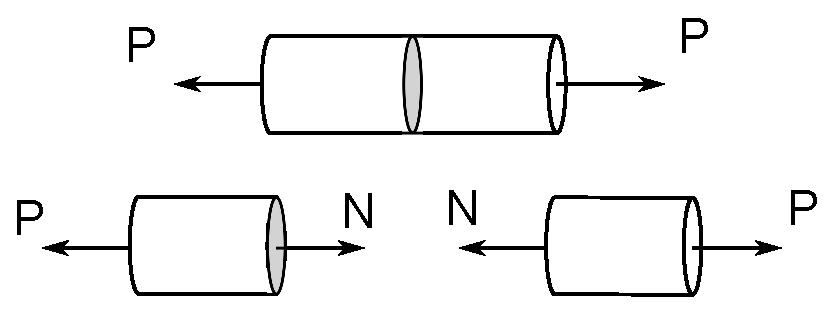
\includegraphics[width = 0.5\textwidth]{./Images/cylinder_forces.eps}
	\caption{Illustration av en stång som utsätts för en dragkraft och de orsakade inre krafterna.}
	\label{fig:cylinder_forces}
\end{figure}

Kraften $P$ i änderna propageras som inre krafter i stången. Om vi betraktar det indikerade tvärsnittet, manifesteras den inre kraften som en normalkraft på varje halva. Om vi definierar positiv riktning för normalkraften och dragkraften som i figuren, ger kraftjämvikten att $N = P$. Om dragkraften blir en tryckkraft, ändrar givetvis normalkraften riktning.

\paragraph{Spänning}
I hållfasthetslära är vi intresserade av påkänningen på materialet. Den beror av beloppet av normalkraften, men kan även spridas ut över tvärsnittet. Därför definierar vi spänningen
\begin{align*}
	\sigma = \frac{N}{A}.
\end{align*}
Jämvikten från innan ger
\begin{align*}
	\sigma = \frac{P}{A}.
\end{align*}

\paragraph{Deformation}
När en stång utsätts för spänning, kommer den att deformeras. Mer specifikt kommer den förlängas med en längd $\delta$. Eftersom förlängningen av varje del kommer från kraftjämvikten mellan normalkraften och dragkraften, kommer förlängningen för en given dragkraft bero av längden. Vi definierar därför töjningen
\begin{align*}
	\varepsilon	= \frac{\delta}{L_{0}}
\end{align*}
där $L_{0}$ är stångens ursprungliga längd.

\paragraph{Typer av samband i hållfasthetslära}
I hållfasthetsläran har vi tre typer av samband:
\begin{itemize}
	\item samband mellan krafter.
	\item samband mellan deformationer.
	\item konstitutiva samband (beskrivar materialbeteende).
\end{itemize}

\paragraph{Hookes lag}
Om man gör dragningsprov på olika material för små deformationer, blir plottet av $\sigma$ mot $\varepsilon$ approximativt linjär. Från detta får vi Hookes lag:
\begin{align*}
	\sigma = E\varepsilon.
\end{align*}
$E$ är elasticitetsmodulen, och beskrivar hur styvt materialet är.

Kombinationen av det vi har tills nu ger
\begin{align*}
	P = \frac{EA}{L}\delta
\end{align*}
för en homogen stång som utsätts för en dragkraft $P$.

Om ett material komprimeras, visar det sig att det elastiska beteendet ofta är likt, med samma elasticitetsmodul.

\paragraph{Normalspänning}
Vi utvidgar våran definition av spänning till spänningar som fördelas inhomogent över tvärsnittet vid att betrakta en inre kraft $\Delta F$ som verkar på ett arealement $\Delta A$, med riktningar som tidigare. Då definieras normalspänningen som
\begin{align*}
	\sigma = \lim\limits_{\Delta A\to 0}\frac{\Delta F}{\Delta A}.
\end{align*}

\paragraph{Normaltöjning}
Vi utvidgar även definitionen av töjning till töjningar som fördelas ojämnt över stavens längd. Om deformationen i en punkt är $u(x)$, ges töjningen av ett litet element med längd $\Delta x$ av
\begin{align*}
	\varepsilon = \lim\limits_{\Delta x\to 0}\frac{u(x + \Delta x) - u(x)}{\Delta x} = \dv{u}{x}.
\end{align*}
Vi ser av detta att töjningen är linjär, så vi kan addera bidrag till den.

\paragraph{Termoelasticitet}
Låt $T$ beteckna en stångs temperatur. En temperaturändring orsakar en termisk töjning
\begin{align*}
	\varepsilon_{T} = \alpha\Delta T,
\end{align*}
där $\alpha$ är längdutvidgningskoefficienten. Man behöver givetvis utgå från en referenstemperatur.

\paragraph{Allmänt enaxligt tillstånd}
Från det vi har sett hittils, kan vi skriva upp en differentialekvation som beskriver det enaxliga tillståndet.

Betrakta en stång med variabel tvärsnittsyta där det överallt i kroppen verkar en volymskraft $K(x)$ (kraft per volym), samt krafter $P_{\text{V}}$ respektiva $P_{\text{H}}$ i varje ända. Vi betraktar ett litet element med tjocklek $\dd{x}$. I ena ändan verkar kraften $K(x)A\dd{x}$ och en normalkraft $N(x)$ på grund av krafterna på volymelementet till vänster, och i andra ändan verkar en normalkraft $N(x + \dd{x})$ på grund av krafterna på volyemelementet till höger.

Kraftjämvikten ger
\begin{align*}
	N(x + \dd{x}) - N(x) + K(x)A\dd{x} &= 0, \\
	\dd{N}{x} + K(x)                   &= 0.
\end{align*}
Vi inför nu definitionen av töjninc och skriver den som en linjärkombination av bidrag från spänning och termoelasticitet, vilket ger
\begin{align*}
	\varepsilon = \frac{\sigma}{E} + \alpha\Delta T, \\
	\sigma = E(\varepsilon - \alpha\Delta T).
\end{align*}
Kombinerad med definitionen av töjning ger det
\begin{align*}
	\dv{x} (\sigma A) + K(x)A &= 0, \\
	\dv{x} (EA(\varepsilon - \alpha\Delta T)) + K(x)A &= 0, \\
	\dv{x}\left(EA\dv{u}{x}\right) + K(x)A &= \dv{x}(EA\alpha\Delta T).
\end{align*}
Detta kommer med randvillkor, och är typiskt randvillkor i deformationen eller i spänningen. Eftersom spänningen är proportionell mot derivatan av deformationen, motsvarar dessa Dirichlet- respektiva Neumannvillkor.

\section{Koncept i tre dimensioner}

\paragraph{Tvärkontraktion}
När man gör ett dragningsprov på en stång, genomgår den deformation i längdriktning samtidigt som tjockleken minskar. Detta kallas tvärkontraktion. Töjningen $\varepsilon_{t}$ av tjockleken är relaterad till töjningen i längdriktning genom
\begin{align*}
	\varepsilon_{t} = -\nu\varepsilon,
\end{align*}
där $\nu$ är Poissons konstant. Termodynamiken ger att $-1\leq\nu\leq 0.5$.

\paragraph{Skjuvspänning}
Betrakta två plattor som ligger på varandra och dras åt motsatta håll av en kraft $F$ på varje. Om de inte dras isär, balanseras dragkrafterna av krafter i kontaktytan. Låt $A$ vara kontaktytan mellan plattorna. Då definieras skjuvspänningen som
\begin{align*}
	\tau = \frac{F}{A}.
\end{align*}

\paragraph{Deformation från skjuvkrafter}
Betrakta ett rätblock med basarea $A$ och höjd $H$ som dras av motsatt riktade krafter med belopp $F$ på varje sida, illustrerad i figur \ref{fig:rectangle_twist}.
\begin{figure}[!ht]
	\centering
	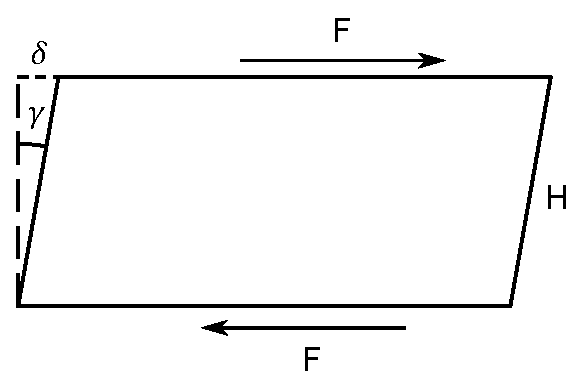
\includegraphics[width = 0.5\textwidth]{./Images/rectangle_twist.eps}
	\label{fig:rectangle_twist}
\end{figure}

Vi kan här definiera skjuvspänningen som
\begin{align*}
	\tau = \frac{F}{A},
\end{align*}
då vi kan tänka oss att plattorna som dras isär är tunna skikt i materialet. Skjuvkrafterna kommer skapa en deformation $\delta$ på en sida motsvarande vridning med en vinkel $\gamma$. Denna vinkeln uppfyller
\begin{align*}
	\tan{\gamma} = \frac{\delta}{H}.
\end{align*}
För små deformationer kan vi approximera
\begin{align*}
	\gamma = \frac{\delta}{H}.
\end{align*}
Experimentellt har man sett att
\begin{align*}
	\tau = G\gamma,
\end{align*}
där $G$ är skjuvmodulen.

\paragraph{Samband mellan materialstorheter}
För ett isotropt material gäller att
\begin{align*}
	G = \frac{E}{2(1 + \nu)}.
\end{align*}

\paragraph{Statiskt bestämta och obestämta problem}
Ett problemt är statiskt bestämt om alla inre krafter och reaktionskrafter kan bestämmas enbart med jämvikt. Detta är möjligt om det verkar maximalt $3$ krafter i planet eller $6$ i rymden.

Om ett problem ej är statiskt bestämt, är det statiskt obestämt. Då räcker icke jämviktsekvationerna, och det motsvarar att man kan ta bort ett element och vara kvar i jämvikt.

\paragraph{Elastisk vridning}
Antag att man har en stång med cirkulärt tvärsnitt fäst i ena ändan som man vrider med ett moment $M_{\text{v}}$ (i varje ända). Detta ger en vinkeldeformation $\theta$ i det yttersta tvärsnittet och $\gamma$ relativt linjen parallellt med stångens riktning. Om stången har en längd $l$ och en radius $a$, ger detta
\begin{align*}
	L\gamma = a\theta.
\end{align*}
Kombinerad med resultatet från delen om skjuvspänning ger detta
\begin{align*}
	\frac{\theta}{L} = \frac{\tau}{G}.
\end{align*}
Antag nu att $\tau = \frac{M_{\text{v}}}{K}$. Detta ger
\begin{align*}
	\frac{\theta}{L} = \frac{M_{\text{v}}}{GK}.
\end{align*}
$K$ är en konstant som beror av stångens geometri.

Hur beräknar vi $K$? Jo, man integrerar momentets differential över tvärsnittet. Vi vet att detta differentialet ges av kraft gånger arm, och det är så skjuvspänningen kommer in.

\paragraph{Balkböjning}
För att beskriva balkar behöver vi införa fler olika sorters inre krafter och moment. Dessa illustreras i figur \ref{fig:beam_forces}.
\begin{figure}[!ht]
	\centering
	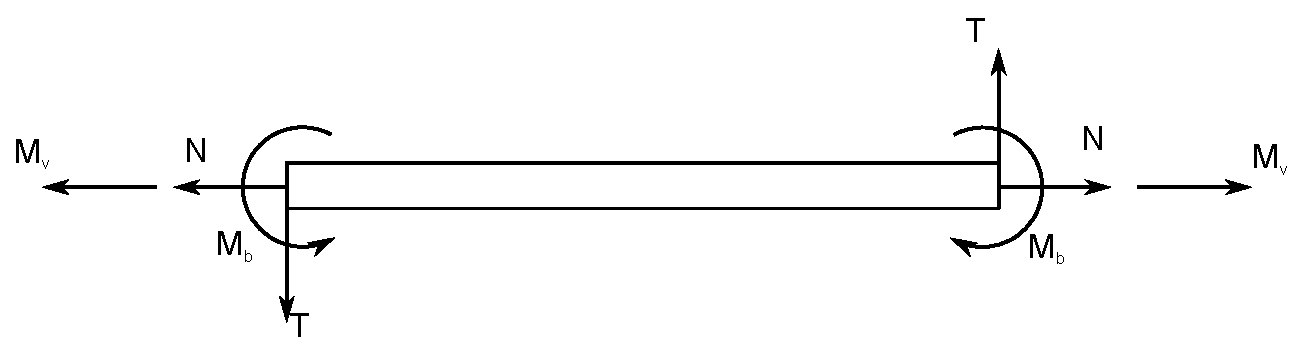
\includegraphics[width = 0.5\textwidth]{./Images/beam_forces.eps}
	\caption{Illustration av inre krafter och moment i en balk.}
	\label{fig:beam_forces}
\end{figure}
Vi har infört normalkraften $N$, tvärkraften $T$, det böjande momentet $M_{\text{b}}$ och det vridande momentet $M_{\text{v}}$.

Låt $u$ vara balkens deformation normalt på dens utsträkning. Vi har från enaxliga tillståndet att
\begin{align*}
	\frac{\Delta u}{L} = \frac{N}{EA}.
\end{align*}
Låt $\theta$ och $\phi$ vara vinklarna för böjning och vridning. Vi har då
\begin{align*}
	\frac{\Delta\theta}{L} = \frac{M_{\text{v}}}{GK},
	\frac{\Delta\phi}{L} = \frac{M_{\text{b}}}{EI}.
\end{align*}

\paragraph{Allmänt tillstånd för en balk}
Snitta nu ut ett element med längd $\dd{x}$ från en balk. Om balken påverkas av en last $q$ per längdenhet, ger kraftjämvikten
\begin{align*}
	T(x + \dd{x}) - T(x) + q(x)\dd{x} = 0,
\end{align*}
vilket ger
\begin{align*}
	\dd{T}{x} = -q.
\end{align*}
Momentjämvikt kring centrum ger
\begin{align*}
	M(x + \dd{x}) - M(x) - (T(x) + T(x + \dd{x}))\dd{x} = 0.
\end{align*}
Bidraget från tvärkraften ges av
\begin{align*}
	T(x) + T(x + \dd{x}) &= 2T(x) + \dv{T}{x}\dd{x} \\
	                     &= 2T(x) - q(x)\dd{x}.
\end{align*}
Insatt i momentjämvikten fås
\begin{align*}
	M(x + \dd{x}) - M(x) - \frac{1}{2}\dd{x}(T(x) + T(x + \dd{x})) = M(x + \dd{x}) - M(x) - T(x)\dd{x} + \frac{1}{2}\dd{x}q(x)\dd{x}.
\end{align*}
Vi försummar nu alla andra ordningens termer, vilket ger
\begin{align*}
	\dv{M}{x} = T.
\end{align*}
Kombinerat med det förra resultatet fås
\begin{align*}
	\dv[2]{M}{x} = -q.
\end{align*}

\paragraph{Randvillkor för balkar}
En balk kan i en given ända vara
\begin{itemize}
	\item fri, vilket ger $T = 0$ och $M = 0$.
	\item fritt upplagd, vilket ger $M = 0$.
	\item glidinspänd, vilket ger $T = 0$.
	\item fast inspönd, vilket ej ger villkor för de inre krafterna och momenterna.
\end{itemize}

\section{Balkar}

\paragraph{Balkböjning - fundamentala koncept}
För att beskriva balkar behöver vi införa fler olika sorters inre krafter och moment. Dessa illustreras i figur \ref{fig:beam_forces}.
\begin{figure}[!ht]
	\centering
	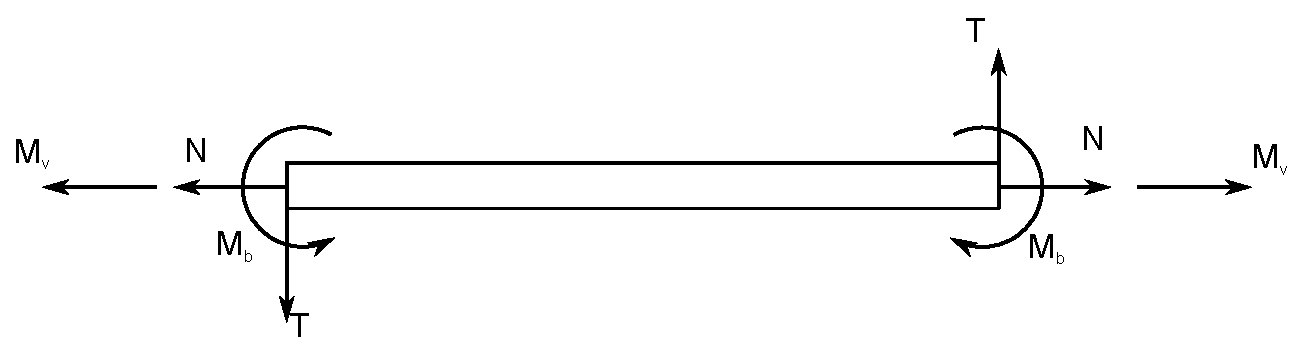
\includegraphics[width = 0.5\textwidth]{./Images/beam_forces.eps}
	\caption{Illustration av inre krafter och moment i en balk.}
	\label{fig:beam_forces}
\end{figure}
Vi har infört normalkraften $N$, tvärkraften $T$, det böjande momentet $M_{\text{b}}$ och det vridande momentet $M_{\text{v}}$.

Låt $u$ vara balkens deformation normalt på dens utsträkning. Vi har från enaxliga tillståndet att
\begin{align*}
	\frac{\Delta u}{L} = \frac{N}{EA}.
\end{align*}
Låt $\theta$ och $\phi$ vara vinklarna för böjning och vridning. Vi har från innan att
\begin{align*}
	\frac{\Delta\theta}{L} = \frac{M_{\text{v}}}{GK},
	\frac{\Delta\phi}{L} = \frac{M_{\text{b}}}{EI}.
\end{align*}

\paragraph{Allmänt tillstånd för en balk}
Snitta nu ut ett element med längd $\dd{x}$ från en balk. Om balken påverkas av en last $q$ per längdenhet, ger kraftjämvikten
\begin{align*}
	T(x + \dd{x}) - T(x) + q(x)\dd{x} = 0,
\end{align*}
vilket ger
\begin{align*}
	\dd{T}{x} = -q.
\end{align*}
Momentjämvikt kring centrum ger
\begin{align*}
	M(x + \dd{x}) - M(x) - (T(x) + T(x + \dd{x}))\dd{x} = 0.
\end{align*}
Bidraget från tvärkraften ges av
\begin{align*}
	T(x) + T(x + \dd{x}) &= 2T(x) + \dv{T}{x}\dd{x} \\
	                     &= 2T(x) - q(x)\dd{x}.
\end{align*}
Insatt i momentjämvikten fås
\begin{align*}
	M(x + \dd{x}) - M(x) - \frac{1}{2}\dd{x}(T(x) + T(x + \dd{x})) = M(x + \dd{x}) - M(x) - T(x)\dd{x} + \frac{1}{2}\dd{x}q(x)\dd{x}.
\end{align*}
Vi försummar nu alla andra ordningens termer, vilket ger
\begin{align*}
	\dv{M}{x} = T.
\end{align*}
Kombinerat med det förra resultatet fås
\begin{align*}
	\dv[2]{M}{x} = -q.
\end{align*}

\paragraph{Randvillkor för balkar}
En balk kan i en given ända vara
\begin{itemize}
	\item fri, vilket ger $T = 0$ och $M = 0$.
	\item fritt upplagd, vilket ger $M = 0$.
	\item glidinspänd, vilket ger $T = 0$.
	\item fast inspönd, vilket ej ger villkor för de inre krafterna och momenterna.
\end{itemize}

\paragraph{Balkböjning vid normalspänning}
Vid böjning inför vi en $z$-koordinat normal på medellinjen genom balken, och centrerar våra koordinater i tvärsnittets tyngdpunkt. Vi antar till att börja med att tvärsnittet är symmetrisk med avseende på $z$-axeln, samt att
\begin{itemize}
	\item plana tvärsnitt förblir plana.
	\item tvärsnitt förblir vinkelräta mot medellinjen.
	\item det för varje $z$ är ett enaxligt samband mellan $\sigma$ och $\varepsilon$.
	\item alla deformationer är små och för balkar vars längd är mycket större än deras tjocklek.
\end{itemize}
De två första uppfylls om skjuvspänningen är försumbar jämförd med normalspänningen.

Betrakta nu ett litet element med ursprunglig längd $L_{0}$ vars medellinje har böjts så den har krökningsradie $R$. Geometri ger oss
\begin{align*}
	(R + z)\phi = L_{0}(1 + \varepsilon(z)).
\end{align*}
I $z = 0$ har vi
\begin{align*}
	R\phi = L_{0}(1 + \varepsilon_{0}),
\end{align*}
vilket ger
\begin{align*}
	L_{0}(1 + \varepsilon_{0}) + z\phi &= L_{0}(1 + \varepsilon(z)), \\
	\varepsilon(z)                     &= \varepsilon_{0} + \frac{\phi}{L_{0}}z.
\end{align*}
Vi kan även substituera för $\phi$ för att få
\begin{align*}
	\varepsilon(z) = \varepsilon_{0} + \frac{1 + \varepsilon_{0}}{R}z.
\end{align*}

Om vi snittar och får någon given normalkraft $N$ på ytan, gäller det att
\begin{align*}
	N &= \integ{A}{}{F}{} \\
	  &= \integ{A}{}{A}{\sigma}.
\end{align*}
Hookes lag ger
\begin{align*}
	N &= \integ{A}{}{A}{E\left(\varepsilon_{0} + \frac{z}{R}\right)} \\
	  &= \integ{A}{}{A}{E\varepsilon_{0} + E\frac{z}{R}}.
\end{align*}
Om vi antar att elasticitetsmodulen är konstant över ytan, kan vi dra ut konstanter. Den andra integralen är då tyngdpunktens $z$-koordinat (om vi antar homogen massfördelning), som per definition var $0$. Detta ger
\begin{align*}
	N = E\varepsilon_{0}A.
\end{align*}

Vi beräknar vidare det böjande momentet $M_{y}$, som är normalt på både längdriktningen och $z$-koordinaten. Detta ges av
\begin{align*}
	M_{y} &= \integ{A}{}{A}{\sigma z} \\
	      &= \integ{A}{}{A}{Ez\left(\varepsilon_{0} + \frac{z}{R}\right)} \\
	      &= \integ{A}{}{A}{Ez\varepsilon_{0} + \frac{E}{R}z^{2}}.
\end{align*}
Första integralen är igen lika med $0$. Andra är relaterad till yttröghetsmomentet
\begin{align*}
	I_{y} = \integ{A}{}{A}{z^{2}}.
\end{align*}
Vi får alltså
\begin{align*}
	M_{y} = \frac{EI_{y}}{R}.
\end{align*}
Vi kan nu sätta ihop dessa resultat och få
\begin{align*}
	\sigma = \frac{N}{A} + \frac{M_{y}}{I_{y}}z.
\end{align*}

Vid ren böjning, dvs. ingen normalkraft, kan vi skriva
\begin{align*}
	\abs{\sigma}_{\text{max}} = \frac{\abs{M_{y}}\abs{z}_{\text{max}}}{I_{y}}.
\end{align*}
Vi kan införa böjmotståndet
\begin{align*}
	W_{\text{b}} = \frac{I_{y}}{\abs{z}_{\text{max}}},
\end{align*}
och får då
\begin{align*}
	\abs{\sigma}_{\text{max}} = \frac{\abs{M_{y}}}{W_{\text{b}}}.
\end{align*}

\paragraph{Allmänt tillstånd för en balk}
Vi försöker nu sammanställa dessa resultat till ett allmänt tillstånd för balken.

Geometri ger oss att
\begin{align*}
	\frac{1}{\abs{R}} = \frac{\dv[2]{u}{x}}{\left(1 + \left(\dv{u}{x}\right)^{2}\right)^{\frac{3}{2}}}.
\end{align*}
För små deformationen är derivatan mycket liten. Om vi definierar positiv krökning som att balken kröks nedåt, fås
\begin{align*}
	\frac{1}{R} = -\dv[2]{u}{x}.
\end{align*}
Materialsamband ger
\begin{align*}
	M_{\text{b}} = -EI_{y}\dv[2]{u}{x}.
\end{align*}
Vi har även
\begin{align*}
	\dv[2]{M_{\text{b}}}{x} = -q,
\end{align*}
vilket slutligen ger
\begin{align*}
	\dv[2]{x}\left(EI_{y}\dv[2]{u}{x}\right) = q.
\end{align*}

Till detta tillståndet hör olika sorters randvillkor. Några enkla varianter av randvillkor är
\begin{itemize}
	\item $u$ eller $T$ givna i ändpunkterna.
	\item $\dv{u}{x}$ eller $M$ givna i ändpunkterna.
\end{itemize}
Vi kan även karakterisera ändpunkter som
\begin{itemize}
	\item fria, dvs. $T = 0$ och $M = 0$.
	\item fritt upplaggda, dvs. $u = 0$ och $M = 0$.
	\item fast inspända, dvs. $u = 0$ och $\dv{u}{x} = 0$.
	\item glidande inspända, dvs. $\dv{u}{x} = 0$ och $T = 0$.
\end{itemize}

\paragraph{Superposition}
Balkens allmänna tillstånd är linjärt, så om man har någon komplicerad sammansättning av yttre laster och krafter, kan man separera problemet i olika delproblem, lösa de separat och superponera lösningen.

\paragraph{Plasticering av balk}
Betrakta en balk som endast utsätts för ett böjmoment $M$. Vid inledande plasticering är
\begin{align*}
	\sigma_{\text{max}} = \sigma_{\text{s}}.
\end{align*}
Vi vet i detta fallet att
\begin{align*}
	\sigma_{\text{max}} = \frac{\abs{M}}{W_{\text{b}}},
\end{align*}
vilket ger
\begin{align*}
	M_{\text{s}} = W_{\text{b}}\sigma_{\text{s}}.
\end{align*}

Vid full plasticering är spänningen lika med $\sigma_{\text{s}}$ i hela balken. Från detta kan man beräkna böjmomentet. Som ett exempel fås för ett rektangulärt tvärsnitt som böjs i höjdriktning:
\begin{align*}
	M_{\text{f}} = 2\cdot\sigma_{\text{s}}b\frac{h}{2}\cdot\frac{h}{4}.
\end{align*}
Man kan även visa att detta är lika med $\frac{3}{2}M_{\text{s}}$.

Vid avlastning kan man använda superposition för att få spänningstillståndet. Det kommer visa sig att restspänningen är diskontinuerlig i mitten.

\paragraph{Tillstånd för axialbelastad balk}
Betrakta en balk som utsätts för en axial belastning, och snitta ut ett element i den enligt figur \ref{fig:skew_beam_forces}.
\begin{figure}
	\centering
	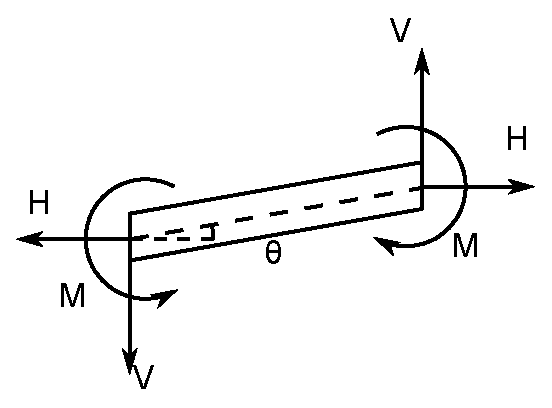
\includegraphics[width = 0.5\textwidth]{./Images/skew_beam_forces.eps}
	\caption{Snitt i en axialbelastad balk, där snittet görs vertikalt relativt det odeformerade läget.}
	\label{fig:skew_beam_forces}
\end{figure}
Kraft- och momentjämvikter ger
\begin{align*}
	V(x + \dd{x}) - V(x) + q\dd{x} = 0, \\
	H(x + \dd{x}) - H(x) = 0, \\
	M(x + \dd{x}) - M(x) - V(x)\dd{x} + H\dv{w}{x}\dd{x} = 0,
\end{align*}
där vi har utnyttjat att vinkeln $\theta$ ges av derivatan av utböjningen och försummat det andra ordningens bidraget till momentet från den utbrädda lasten. Detta ger
\begin{align*}
	\dv{V}{x} = -q,\ \dv{H}{x} = 0,\ \dv{M}{x} = V - H\dv{w}{x}.
\end{align*}
Man kan visa att till första ordningen är $H = N$, och $N$ ges av den yttre axiala lasten (och eventuella volymkrafter). Kombinationen av dessa ekvationer ger då
\begin{align*}
	\dv[2]{x}\left(EI\dv[2]{w}{x}\right) - N\dv[2]{w}{x} = 0.
\end{align*}

\section{Analys i tre dimensioner}

\paragraph{Spänning}
Vi definierar spänningsvektorn
\begin{align*}
	\vb{s} = \lim\limits_{A \to 0}\frac{\vb{F}}{A}
\end{align*}
där $\vb{F}$ är kraften på det lilla arealementet. Den har en komponent normalt på ytan, som är normalspänningen, och en komponent som är parallel med ytan, som är skjuvspänningen. Vi får
\begin{align*}
	\sigma = \vb{s}\cdot\vb{n}, \tau^{2} = \abs{\vb{s}}^{2} - \sigma^{2}.
\end{align*}

\paragraph{Skjuvspänningar i tre dimensioner}
Snitta nu ut en infinitesimal kub. På ytorna, till exempel ytan som är normal på $x$-axeln, kan man dekomponera spänningsvektorn i en normalspänning $\sigma_{x}$ och två skjuvspänningar $\tau_{xy}, \tau_{xz}$, och motsvarande i andra riktningar. Om vi tittar på momentjämvikt kring kubens centrum i $x$-riktning fås
\begin{align*}
	2\tau_{yz}\dd{x}\dd{z}\cdot\frac{1}{2}\dd{y} - 2\tau_{zy}\dd{x}\dd{y}\cdot\frac{1}{2}\dd{z}        &= 0, \\
	\tau_{yz} &= \tau_{zy}.
\end{align*}
En motsvarande härledning kan göras för de andra sidorna. Tillkommer det andra termer om skjuvspänningen varierar? Ja, men dessa kommer vara av högre ordning, och kan försummas.

\paragraph{Spänningsmatris}
Vi kan nu definiera en spänningsmatris
\begin{align*}
	S =
	\mqty[
		\sigma_{x} & \tau_{yx}  & \tau_{zx} \\
		\tau_{xy}  & \sigma_{y} & \tau_{zy} \\
		\tau_{xz}  & \tau_{yz}  & \sigma_{z}
	].
\end{align*}
Enligt argumentet ovan är denna symmetrisk.

\paragraph{Spänningar på godtycklig yta}
Om man har en godtycklig yta med normalvektor $\vb{n}$, kan det visas att spänningarna på ytan ges av
\begin{align*}
	\vb{s} = S\vb{n}.
\end{align*}
Vi kan då skriva
\begin{align*}
	\sigma &= \vb{n}^{T}S\vb{n}, \\
	\tau   &= \abs{S\vb{n}}^{2} - (\vb{n}^{T}S\vb{n})^{2}.
\end{align*}

\paragraph{Huvudspänningar}
Finns det orienteringar sådana att $\vb{s} = \sigma\vb{n}$? Att hitta sådana är ett egenvärdesproblem. Matematiken ger att det finns sådana orienteringar, och att de är ortogonala mot varandra.

\paragraph{Plana tillstånd}
Ett specialfall är när $z$-riktningen är en huvudriktning för spänningen. Då är skjuvspänningarna i $xy$-planet, dvs. $\tau_{zx} = \tau_{zy} = 0$. Om $\sigma_{z} = 0$, har man plan spänning.

Betrakta plan spänning på ett plan som bildar en vinkel $\phi$ med $y$-axeln. Normalvektorn ges av
\begin{align*}
	\vb{n} = \cos{\phi}\vb{e}_{x} + \sin{\phi}\vb{e}_{y}.
\end{align*}
Vi får då
\begin{align*}
	\sigma &= \sigma_{x}\cos[2]{\phi} + \sigma_{y}\sin[2]{\phi} + 2\tau_{xy}\sin{\phi}\cos{\phi}, \\
	\tau   &= \tau_{xy}\cos{2\phi} + \frac{\sigma_{y} - \sigma_{x}}{2}\sin{2\phi}.
\end{align*}

\paragraph{Mohrs spänningscirkel}
Mohrs spänningscirkel är ett sätt att grafiskt ta fram plana spänningar vid rotation av ett plan. För att konstruera cirkeln, rita upp ett $\sigma, \tau$-koordinatsystem och två punkter $(sigma_{x}, \tau_{x, y})$ och $(sigma_{y}, -\tau_{x, y})$, där dessa tas från något givet tillstånd. Dessa punkter skall vara i motstående änder av cirkeln, och från detta kan cirkeln ritas. En rotation moturs av planet med en vinkel $\phi$ motsvarar en rotation medurs av tillståndet på cirkeln med en vinkel $2\phi$.

\paragraph{Jämvikt i tre dimensioner}
Snitta ut en liten kub. Jämvikt i $x$-riktning ger
\begin{align*}
	\sigma(\vb{x} + \dd{x}\vb{e}_{x})\dd{y}\dd{z} - \sigma(\vb{x})\dd{y}\dd{z} + \tau_{zx}(\vb{x} + \dd{z}\vb{e}_{z})\dd{x}\dd{y} - \tau_{zx}(\vb{x})\dd{x}\dd{y} + \tau_{yx}(\vb{x} + \dd{y}\vb{e}_{y})\dd{x}\dd{z} - \tau_{yx}(\vb{x})\dd{x}\dd{z} = 0,
\end{align*}
vilket implicerar
\begin{align*}
	\del{x}{\sigma_{x}} + \del{y}{\tau_{xy}} + \del{z}{tau_{zx}} = 0.
\end{align*}


\section{Materialers beteende}

\paragraph{Idealplastisk deformation}
De flesta material beter sig så att när de deformeras förbi en viss punkt, deformeras de plastiskt i stället för elastiskt. En approximation för att beskriva detta beteendet är att låta deformationen vara elastisk upp till en töjningsgräns $\varepsilon_{\text{s}}$, och låta $\sigma$ vara konstant lika med en sträckgräns $\sigma_{\text{s}}$ för större töjningar.

Om materialet komprimeras, visar det sig att det elastiska beteendet ofta är likt.

När lasten sedan tas bort, kommer stången förkortas igen tills lasten blir lika med noll. Denna kontraktionen är parallell med det elastiska regimet, och konsekvensen är att man får en permanent deformation.

\end{document}
